\fancyhead{}
\fancyfoot{}
\newtheorem{teorema}{Teorema}

\lhead{Conceptos fundamentales, teor�as y antecedentes}
%\rhead{\today}
%\rfoot{\thepage}

\section{Resultado del Diagn�stico.}
Dar un soluci�n rapida a los problemas de servidores, en especial cuando estas est�n en alguna regiones donde el acceso se hace dif�cil, ya sea por inclemencia de tiempo o alg�n otro factor, puede provocar que no se pueda poner el linea a estos, por d�as e inclusive semanas, dejando a las unidades sin funcionamiento. ya que resulta mas f�cil para el usuario com�n conectarse desde otra m�quina en algun lugar con conexi�n a \Gls{internet}, que intentar reparar el servidor.
\subsection{Planteamiento del Problema}
El problema que se desea solucionar es la perdida la de se�al entre la central y las filiales, la replicaci�n de los datos. Como se muestra en la (Fig. \ref{situacion-actual}), cada sucursal tiene su propio servidor, dificultando la replicaci�n de los datos a los servidores de la central\\
\begin{figure}[H]
\begin{center}
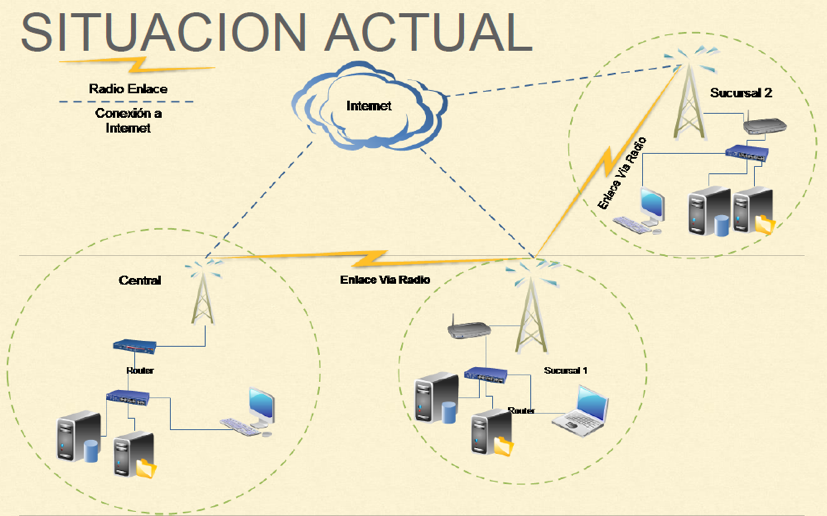
\includegraphics[scale = .8]{figuras/figura003.png}
\caption{Situacion Actual, donde cada filial tiene un servidor para cada servicio.}
\label{situacion-actual}
\end{center}
\end{figure}
Una vez realizado la conexi�n por medio de tuneles redundates, como se puede ver en la (Fig. \ref{situacion-esperada}), los datos quedan almacenado en el servidor de la central, de esta manera reducir al minino los problemas de incoherencia a causas de replicaciones.\\
\begin{figure}[H]
\begin{center}
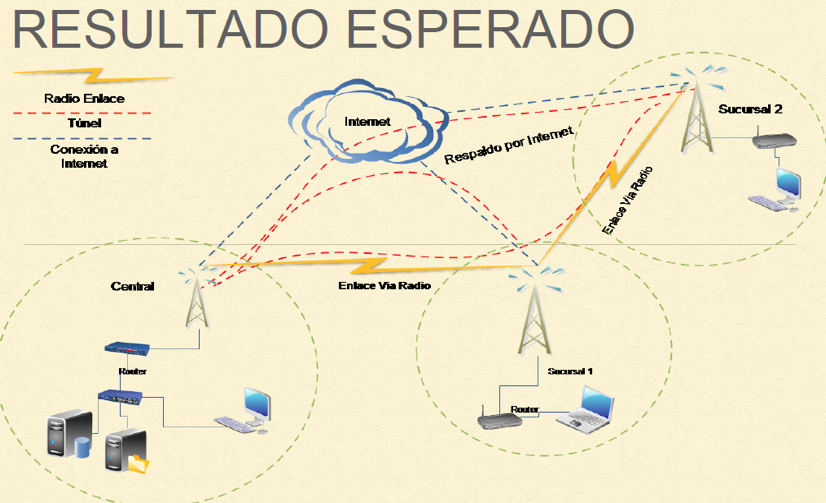
\includegraphics[scale = .8]{figuras/figura004.png}
\caption{Situacion Esperada, con la implementacion de los tuneles redundates, los servidores quedan centalizados.}
\label{situacion-esperada}
\end{center}
\end{figure}
\section{Antecedentes}
La importancia de la tecnolog�a de las redes de datos para las comunicaciones en las organizaciones (empresas, instituciones gubernamentales, no gubernamentales) ha sido fundamental para su desarrollo y crecimiento, tanto en el aspecto econ�mico y funcional, siendo una herramienta estrat�gica que brinda soporte y permite el desenvolvimiento y transformaci�n de dichas organizaciones. Hoy en d�a no se puede concebir, a nivel organizacional, alg�n cambio, fusi�n u uni�n sin considerar las comunicaciones y las tecnolog�as de informaci�n que le dan soporte.\\
Ya se realizaron varios trabajos relacionados a \Gls{vpn}, cada una de ellas con sus particularidades. 
Cabe destacar \textit{``Redes VPNs de Acceso Remoto''}, realizado por Mario Rub�n Mansilla y Eduardo Rodolfo Colombres, donde los objetivos generales fueron: Investigar las caracter�sticas, componentes, mecanismos de una VPN de acceso remoto y como solucionan la necesidad de un ingreso seguro a los recursos inform�ticos de la organizaci�n desde cualquier sitio y Aplicar los conceptos de VPN de acceso remoto a trav�s de una soluci�n que implemente un cliente VPN port�til que evite la instalaci�n de programas para esta tarea.\cite{red:vpn}
\textit{``Las comunicaciones en las redes privadas virtuales''} de Jes�s y Juan Hern�ndez donde el objetivo principal es implementar VPN en una plataforma Windows.\cite{protocolo:2003}
En otro trabajo similar, \textit{``Estudio e implementaci�n de un radio enlace con tecnolog�a mikrotik para el ISP Sistemas en el cant�n gualaquiza, provincia morona santiago''}, de Klever Mauricio Suqui Carchipulla . Estos autores estudian las propiedades de los radios enlaces a profundidad.\cite{suqui:2010}